\section{阻抗}
\label{sec:4.6}

经典物理学非常注意能量守恒与耗散问题,工程滤波理论非常注意时间因果性问题、即
激发之前不可能存在响应。在地球物理学中,我们经常需要既能保证时间因果性关系,又要
考虑能量损耗的问题。我们需要不但是在理论推导方面而且在计算方面将二者结合起来,有
时在时间离散化的计算中也需如此。有专门一类称怍阻抗函数的数学函数可用以描述在耗散
能量之物理物体中的因果性线性扰动。

大自然是按时间向前推移发展的。很自然,阻抗函数在任何模拟计算中都是起基本作用
的,在那里,时间是从过去向未来推移发展的。除了它们在物理模拟中的应用以外,阻抗在波
场的深度外推中也发现有用处。地球物理学家将地表面上获得的数据向下外推,以期获得深
处的信息,这种作法不同于大自然沿时间的外推。在原理上,我们并不要求将阻抗函数向深
处外推,但是进行深度偏移而不考虑阻抗函数却会出现不断増大的振荡现象,这一点同接受
外部来源能量的物理系统非常相像。事实上,物理方程的“直接”实现往往表现为不稳定的
外推,若用阻抗函数来表示我们的外推问题,那我们就能保证稳定性。在一种算法所能具有
的一切长处,如稳定性、精度、清晰性、普遍性、效率、模块性等等之中,最为重要的看来
就属稳定性了。

在本节中,我们要研究阻抗函数理论,研究其精确定义、及其离散时间域内的计算方
法、以及由简单阻抗组合成更复杂阻抗函数的规律;我们还要研究其他一些特殊函数、如极
小相位滤波与反射率滤波(reflectance filter)等与阻抗滤波的关系。时间域内的广角波场
外推与偏移将以阻抗函数来表示。岩石因其含有一切尺度的不规则性而与“纯”物质不相
像,我们将求出一种特别简单的阻抗函数来模仿岩石内的能量耗散,它不同于经典的牛顿粘
滞性方程。

\subsection{谨防得出无穷大结果}
\label{sec:4.6.1}

取一个无穷级数,如1,
-1、+1、-1、+1$\ldots\ldots$,以两种不同方式将级数各读组合并
按下列方式将它们相加,可以得出1等于0的荒谬结果:
\begin{equation*}
(1-1)+(1-1)+(1-1)+...=1+(-1+1)+(-1+1)+...
\end{equation*}
\begin{equation*}
0+0+0+...=1+0+0+...
\end{equation*}
当然,这并非真正证明一等于零,而只是证明对无穷级数必须很小心地处理而已。其次,再
取另一种无穷级数,其中各项应可按任意顺序重新分类组合而无需担心得出似是而非的结
果.要得到这类级数,可这么设想:把一个馅饼一分为二,将其中一半再一分为二,得到两
个四分之一的饼,然后再将其中一个四分之一分成两个八分之一的饼$\ldots$,就如此进行下去。
这样的无穷级数就是1/2、1/4、1/8、1/16......,不论把已被分为小块的焰饼如何重新排
列,它们应该总能放回到盛馅饼的盘子内,并准确地把它填满。

无穷级数的危险并不在于它们有无限多项,而在于将它们求和可得出无穷大结果。如果
各项绝对值之和为有限,那就能保证没事,这样一类级数称作绝对收敛级数。

\subsection{Z变换}
\label{sec:4.6.2}


任意离散时间函数$x_t$之Z变换定义为
\begin{equation}
X(Z)=......x_{-2}Z^{-2}+x_{-1}Z^{-1}+x_0+x_1Z+x_2Z^2
\label{eq:ex4.6.1}
\end{equation}
在物理上可把变量Z解释为有一个单位时间的时延,于是之$Z^2$就代表有两个单位时间的延迟,
等等。像$X(Z)U(Z)$和$X(Z)U(1/Z)$这样的表达式在以后是很有用处的,因为它们
的意思是指时间域系数的褶积和互相关(见《地球物理数据处理基飿》一书)。

再往下考虑延迟算子$Z$的数值,我们发现,很有用的是问一下$X(Z)$究竟是有限的还是
无限的。算子$Z$具有特殊意义的数值是$Z=+1$和$Z=-1$,以及$Z$具有单位幅度$\mid Z\mid =1$
的所有复数值,或即
\begin{equation}
Z=e^{i\omega \Delta t}
\label{eq:ex4.6.2}
\end{equation}

式中,$\omega$为Fourier变换的实变量。取$\omega$为实数意味着Z是在单位圆上,这时的Z变换是一种
离散Fourier变换。由于我们要求$U(Z)$对单位圆$\mid Z\mid=1$上的所有Z值均为有限,我们可将
注意力局限于具有有限能量的时间函数。滤波函数总是局限于具有有限能量的。

说滤波是具有因果性,其最直接了当的说法就是说它的时间域系数在零时间以前均等于
零,亦即对于$t<0$应有$u_t=0$;另一种说法就是说,对于$Z=0$,$U(Z)$
应有限。如若各系数
$u_{-1}$、$u_{-2}$...等等不为零,则在Z=0时该$Z$变换将为无限大。对于一个具有因果性的函数,当
Z取在单位圆内$\mid Z\mid<1$而不是取在单位圆$\mid Z\mid=1$上时,$\mid U(Z)\mid$的各项均将比较小,所以
在$Z=0$时和在单位圆$\mid Z\mid=1$上时具有收敛性就是暗示在单位圆内应处处收敛。因此,将有
界性同因果性结合起来就是意味着在单位圆内收敛。在$Z=0$时收敛而在单位圆上$\mid Z\mid=1$不
收敛的情形,属于具有无限能量的因果性函数,这种情形没有实用意义。什么种类的函数是
在单位圆上和在$Z=\infty$时收敛而在$Z=0$时不收敛?什么函数是在所有Z=0、$Z=\infty$和$\mid Z\mid=1$
这三种情形下均收敛?

滤波算子$1/(1-2Z)$至少可按两种不同方式展为Z的幂级数,这两种方式为:
\begin{equation}
\frac{1}{1-2Z}=1+2Z+4Z^2+8Z^3+...\\
=-\frac{1}{2Z}\frac{1}{1-\frac{1}{2Z}}=\frac{-1}{2Z}[1+\frac{1}{2Z}+\frac{1}{4Z^2}+......]
\label{eq:4.6.3}
\end{equation}
这两种无穷级数中哪一种的收敛是与Z的数值有关?对于$\mid Z\mid=1$来说,第一种级数发散,但
第二种级数却收敛,所以,仅有反因果性滤波才是可接受的滤波。级数展开
是唯一的吗?如果收敛,它就是唯一的,复变函数理论可以证明这个结论。

设以$b_t$表示某一滤波器,如果$b_t$与$a_t$的褶积结果是$\delta$函数,则$a_t$就是$b_t$的反滤波器,在
Fourier域内我们就说,如其Fourier变换彼此可逆,则两个滤波器就彼此可逆。反滤波可用
Z变换定义,例如$A(Z) =1/B(Z)$。滤波$A(Z)$是否具有因果性就看它是否在单位圆内
处处有限,或者说,实际是与$B(Z)$是否在单位圆内任何处均等于零有关。例如$B(Z)=1-2Z$在$Z=1/2$时为零,此时$A(Z)=1/B(Z)$必然为无穷大,就是说,级数$A(Z)$在
$Z=l/2$时必然不收敛,因而$a_t$不具有因果性。当滤波$B(Z)$及其倒数均具因果性时,出现
一种最有意义的情形,称为极小相位,以上所述可总结如下:
\begin{table}[!ht]
\centering
\ttfamily
\small
\begin{tabularx}{\textwidth}{Y|Y}
\hline
因果性& $\mid B(Z)\mid<\infty 当\mid Z\mid \le 1$\\
\hline
因果性倒数& $\mid 1/B(Z)\mid<\infty 当\mid Z\mid \le 1$\\
\hline
极小相位 &满足上述两项条件 \\
\hline
\end{tabularx}
\end{table}

\subsection{阻抗滤波器评述}
\label{sec:4.6.3}

利用Z变换的记号定义一种滤波$R(Z)$,其输入为$X(Z)$,其输出为$Y(Z)$,于是
\begin{equation}
Y(Z)=R(Z)X(Z)
\label{eq:ex4.6.4}
\end{equation}
如$R(Z)$的级数形式表示式没有Z的负幂项,就说该滤波是因果性滤波。换句话说,$y_t$可根
据$x_t$的过去值与现在值确定。再者,如$l/R(Z)$不含Z的负幂项,则该滤波$R(Z)$为极小
相位的,这意味着,采用直接的多项式除法
\begin{equation}
X(Z)=\frac{Y(Z)}{R(Z)}
\label{eq:4.6.5}
\end{equation}
即可根据$y_t$的现在值与过去值决定$x_t$。

设$R(Z)$已经是极小相位,若正值的能量或功可表示如下:
\begin{subequations}
\begin{equation}
0\le \text{功}=\sum_t \text{力}\times\text{速度}=\sum_t\text{电压}\times\text{电流}
\label{eq:ex4.6.6a}
\end{equation}
\begin{equation}
=\frac{1}{2}\sum_t(\bar{x_t}y_t+\bar{y_t}x_t)
\label{eq:ex4.6.6b}
\end{equation}
\begin{equation}
=[\bar{X}(\frac{1}{Z})Y(Z)+\bar{Y}(\frac{1}{Z})X(Z)]\text{的}Z^0\text{项之系数}
\label{eq:ex4.6.6c}
\end{equation}
\begin{equation}
=\frac{1}{2\pi}\int_0^{2\pi}Re(\bar{X}Y)d\omega
\label{eq:ex4.6.6d}
\end{equation}
\begin{equation}
=\int Re(\bar{X}RX)d\omega =\int \bar{X}X Re(R)d\omega
\label{eq:ex4.6.6e}
\end{equation}
\end{subequations}
则$R(Z)$还可以是一种阻抗函数。既然$\bar{X}X$可以是位于任何频率$\omega$
上的脉冲函数,从而可以得结论:$Re[R(\omega)]\ge 0$对于所有实数的
$\omega$均成立。以上所述可总结如下:
\begin{table}[!ht]
\centering
\ttfamily
\small
\begin{tabularx}{\textwidth}{Y|Y}
\hline
因果性& $r_t=0$,对于$t<0$即$\mid R(Z)\mid<\infty$,对于$\mid Z\mid \le 1$\\
\hline
因果性倒数& $\mid 1/R(Z)\mid<\infty 当\mid Z\mid \le 1$\\
\hline
耗散能量 &$2ReR(\omega)=R(Z)+\bar{R}(1/Z)\geq 0$,$\omega$为实数 \\
\hline
\end{tabularx}
\end{table}


将阻抗函数与其Fourier共轭函数相加,得出一种像功率谱一般的实数正依函数(其虚
部等于零),例如 
\begin{subequations}
\begin{equation}
(r_0+r_1Z+r_2Z^2+...)+(\bar{r_0}+\bar{r_1}\frac{1}{Z}+\bar{r_2}\frac{1}{Z^2}
+...) \geq 0, \text{对实数$\omega$}
\label{eq:ex4.6.7a}
\end{equation}
\begin{equation}
R(Z)+\bar{R(\frac{1}{Z}}\geq 0, \text{对实数$\omega$}
\label{eq:ex4.6.7b}
\end{equation}
\label{eq:ex4.6.7}
\end{subequations}


\subsection{因果性积分}
\label{sec:4.6.4}

设有离散时间函数其Fourier变换经代换$Z=exp(i\omega \Delta t)$之后,得Z变换为
\begin{equation}
P(z)=......+P_{-2}Z^{-2}+p_{-1}Z^{-1}+p_0+p_1Z+p_2Z^2+......
\label{eq:ex4.6.8}
\end{equation}
根据以下的关系,定义一个算子$-i\hat{\omega}$
\begin{equation}
\frac{1}{-i\hat{\omega}\Delta t}=\frac{1}{2}\frac{1+Z}{1-Z}
\label{eq:ex4.6.9}
\end{equation}
将此算子应用于$P(Z)$,定义出另一个离散时间函数$q_t$,其Z变换为Q(Z)
\begin{equation}
Q(Z)=\frac{1}{2}\frac{1+Z}{1-Z}P(Z)
\label{eq:ex4.6.10}
\end{equation}
两端乘以$(1-Z)$,得
\begin{equation}
(1-Z)Q(Z)=\frac{1}{2}(1+Z)P(Z)
\label{eq:ex4.6.11}
\end{equation}
令两端同幂项$Z^t$的系数相等,则得
\begin{equation}
q_t-q_{t-1}=\frac{p_t+p_{t-1}}{2}
\label{eq:ex4.6.12}
\end{equation}
令$p_t$为脉冲函数,我们就可看出$q_t$原来是一种阶跃函数,即
\begin{subequations}
\begin{equation}
p=......,0,0,0,0,0,1,0,0,0,0,0,......
\label{eq:ex4.6.13a}
\end{equation}
\begin{equation}
q=......,0,0,0,0,0,\frac{1}{2},1,1,1,1,1,......
\label{eq:ex4.6.13b}
\end{equation}
\label{eq:ex4.6.13}
\end{subequations}

因此,$q_t$就是$p_t$从负无限大至时间t之积分的离散时间域表示式,它正好与微分方程
$dQ/dt=P$的Crank-Nicolson型数值积分相同。算子$(1+Z)/(1-Z)$称为双线变换,
对其分子项与分母项各乘以$Z^{-0.5}$并以$Z=e^{i\omega \Delta t}$代入,即可知
对微分作近似时的精度
\begin{subequations}
\begin{equation}
-i\frac{\hat{\omega}\Delta t}{2}=\frac{1-Z}{1+Z}=\frac{Z^{-0.5}-Z^{+0.5}}{Z^{-0.5}+Z^{+0.5}}
\label{eq:ex4.6.14a}
\end{equation}
\begin{equation}
=-i\frac{\sin(\omega \Delta t/2)}{\cos(\omega \Delta t/2)}=-i\tan(\frac{\omega\Delta t}{2})
\label{eq:ex4.6.14b}
\end{equation}
\label{eq:ex4.6.14}
\end{subequations}

该积分算子$(1 + Z)/(1 — Z)$在上有极点,极点正位于单位圆上,这就产生了出现无限大谬误的可能性。换言之,还存在有可作其他形式的非因果性展开的可能。例如,取$1/( —i\omega )$为$\omega$的虚数反对称函数,就是暗示存在有实数的反对称时间函数$sgn(t)=t/\mid t\mid$,而这通常是不能看作积分算子的。为避免任何意义模糊,我们在这里引入一项很小的正数$\epsilon$并定义$\epsilon =l—\rho$,使积分算子变为
\begin{subequations}
\begin{equation}
I=\frac{1}{2}\frac{1+\rho Z}{1-\rho Z}=\frac{1}{2}(1+\rho Z)
[1+(\rho Z)+(\rho Z)^2+(\rho Z)^3+...]
\label{eq:ex4.6.15a}
\end{equation}
\begin{equation}
=\frac{1}{2}+(\rho Z)+(\rho Z)^2+(\rho Z)^3+...
\label{eq:ex4.6.15b}
\end{equation}
\label{eq:ex4.6.15}
\end{subequations}
因为$\rho$比1稍小,这个级数对单位圆上的任何Z值均为收敛;若$\epsilon$为微小的负值而不是正值,则
应将这种展开式表示为Z的负幂而不用正幂。

现在的一铧大好事是,具有时间因果性的积分算子就是阻抗函数的一个例子。该算子很
显然是遵守因果性的,且其逆亦具因果性。让我们检查一下,在频率域内其实部是否为正
值。使分母项有理化,得
\begin{subequations}
\begin{equation}
I=\frac{1}{2}\frac{1+\rho Z}{1-\rho Z}\frac{1-\rho Z}{1-\rho Z}=
\frac{(1-\rho^2)+\rho(Z-1/Z)}{(\text{正值项})}
\label{eq:ex4.6.16a}
\end{equation}
\begin{equation}
=\frac{(1-\rho^2)-i2\rho\sin\omega\Delta t}{(\text{正值项})}
\label{eq:ex4.6.16b}
\end{equation}
\label{eq:ex4.6.16}
\end{subequations}
由此又一次看到,正因为选取一个正使得$(1-\rho^2)$已成为正值,从而使实部对所有频率
$\omega$均为正值,如图\ref{fig:crft/cintegral}所示。

\begin{figure}[H]
\centering
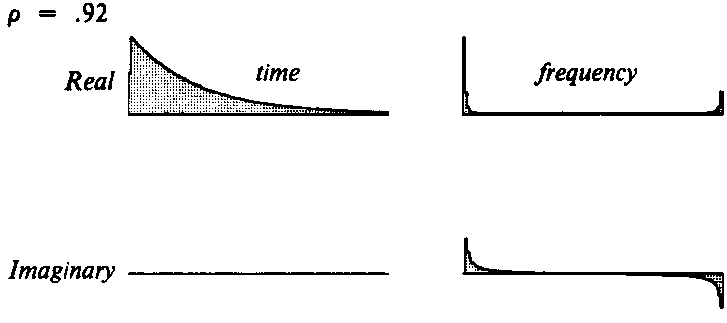
\includegraphics[width=0.65\textwidth]{crft/cintegral}
\caption[cintegral]{时间因果性之积分算子I。频率轴上的曲线代表
256个点上的离散Fourier变换,零时间及零频率各位于其相应坐标轴
之左端。}
\label{fig:crft/cintegral}
\end{figure}

在频率域内乘以$-i\omega$,相应
于时间域内进行微分运箅$d/dt$;
除以$-i\omega$则相应时间域内进行积分运算。人们通常都认为非对称算子$(1,-1)$
相应于时间域的微分运算,但要注意,因果性积分算子的倒数、即
\begin{equation}
I^{-1}=2\frac{1-\rho Z}{1+\rho Z}=2-4\rho Z+4(\rho Z)^2-4(\rho Z)^8+
......
\label{eq:ex4.6.17}
\end{equation}
也代表微分运算,尽管它完全具有因果性而且全然不是非对称的。在线性系统分析中,离散
微分的这种表示式是经常采用的一种形式,构制高阶稳定微分方程要遵守阻抗组合的一定规
则。

偶而需要使微分算子具有负实部,为达此目的,可取$\epsilon$为负值,这意味着要取$\rho>1$,然
后以的幂次作无穷级数展开,就是说,它应是反因果性的而不是因果性的;无论在反因
果性情形或因果性情形下,虚部仍将是$-i\omega$,而实部则将具有与此相反的符号。


\subsection{阻抗组合的Muir规则}
\label{sec:4.6.5}

每一种能量守恒或能量耗散的物理系统都有其阻抗函数,阻抗函数是微分算子与正值物
理常量的特种组合。我们要看一看什么样的组合才是允许的。

要想保证计算过程稳定,重要的是要能够保证假定的阻抗函数确实是一种阻抗函数。应
用地球物理学有这么一种困难:虽然你也许要求所得结果只是遍及有限频率范围,而且你能
够作的近似在那种范围之内也是合理的,可是如果所计算出的阻抗超出该应用范围而变成负
值(接近Nyquist频率时往往出现这种情形),那末阻抗滤波器就会产生数值发散的输出。
因此,即使阻抗几乎就是正确的,也没法采用它。

为将简单阻抗进行组合以得出更复杂的一些阻抗,Francis Muir曾提出三条规则\footnote{
据Francis Muir私人通信。---原注}
这些规则所以特别有用,是因为我们据此可以从微分算子和积分算子的离散时间形式出发进
行讨论。令$R'$表示由已知阻抗函数R及、$R_1$与$R_2$所产生的一个新的阻抗函数,将阻抗组合起
来有三种途径:
\begin{enumerate}
\item 乘以正值标量a $R'$=aR
\item 倒数         $R'=\frac{1}{R}$
\item 加法         $R'=R_1+R_2$
\end{enumerate}

这些规则不包括阻抗函数彼此相乘,不允许乘法是因为要避免出现平方,例如,采用平
方就会使相位角加倍,从而可能破坏实部的正值性。既然这些规则不包括乘法而只是求和、
求倒数和按比例放大或缩小,于是按本来面貌出现的阻抗函数将总是在数学上被表示为连分
式形式。

Muir的头两条规则非常明确,我们将不再证明它们,第三条规则则值得很仔细地注意。
要证明任何规则,我们都需要指明有关的三件事,即它遵守时间因果性,它是正实的
(Fourier变换有正的实部),以及它是可逆的。这最后一部分是Muir的第三条规则的难
题,即两个阻抗之和应具有遵守时间因果性的倒数,证明这件事实得写大约两页纸,并且要
引入若干附加的概念才行。

\subsection{根据反射率定义的阻抗}
\label{sec:4.6.6}

被称为阻抗的一类滤波其范围是很大的,因为阻抗均由易于说明的、被称作反射率的滤
波族$c_t$及其Fourier变换$C(\omega)$经过转换而导出。作为反射率的时间函数必须是严格因果性
的,而且频率函数必须严格小于1。所谓严格因果性是指:时间函数在零时间和零时间以前
都等于零。例如,取$-1<\rho<+1$且反射率$c_t$为某一时刻$\Delta t$之后其幅度为$\rho$的脉冲,其Fourier变换为
\begin{equation}
C=\rho Z=\rho e^{i\omega\Delta t}
\label{eq:ex4.6.18}
\end{equation}
显然,两个反射率之乘积应等于另一个反射率。

阻抗已定义为具有因果性倒数之因果性滤波且其Fourier变换具有正实性(实部为正)
之后,将可证明:根据任何反射率C,可由下列表达式形成一种阻抗R
\begin{equation}
R=\frac{1-C}{1+C}
\label{eq:ex4.6.19}
\end{equation}
有三件事要证明:遵守时间因果性,具有因果性倒数,且为正实性。第一种性质成立是因
为假设幅度严格小于1,即$C\bar{C}<1$,因而分母项可展为收敛级数$1 + C +
C^2+\ldots\ldots$。第二种性质
成立是因为直接改变C的符号即可求出$R$的倒数。将分子与分母均乘以复共轭$(1+\bar{C}$,则
\begin{subequations}
\begin{equation}
ReR=Re[\frac{(1-C)(1+\bar{C})}{\text{正值项}}]\geq 0
\label{eq:ex4.6.20a}
\end{equation}
\begin{equation}
ReR=Re[\frac{(1-C\bar{C})+\text{虚部}}{\text{正值项}}]\geq 0
\label{eq:ex4.6.20b}
\end{equation}
\end{subequations}
这表明第三种性质成立,即R具有的实部为正值。

由及$R(C)$的表达式很容易反向求出$C(R)$的表达式,但由每个R均产生一反射率这种
反定理却较难话明。不过,采用一个较深刻的定理将能证明它。一个滤波既是因果性的又是
上正实性的,就说它是正实因果性CPR的(causal and positive real);该较深刻的定理就
是:每种CPR滤波均具有倒数,因而也就是一种阻抗。指出下列一点就能证明这个定理:
每个具有正实因果性的$\hat{R}$均可用以构制出反射,既然$\hat{R}$是一
种反射率,那末这就是暗示具
有正实因果性的$\hat{R}$即足一种阻抗$R$,于是反解求出
\begin{equation}
\hat{C}=\frac{1-\hat{R}}{1+\hat{R}}
\label{eq:ex4.6.21}
\end{equation}

证明要求表明两件事。第一,$\hat{C}$的幅度小于1;为证实这点,取分母$(1+\hat{R})$
的幅度并从中减去分子$(1-\hat{R})$的幅度,所得结果等于四乘$\hat{R}$的实部,这是个正数
$4Re\hat{R}\geq 0$。第二,
必须证明$\hat{C}$有时间因果性。这点比较难证明;可以把分母$(1+\hat{R})^{-1}$展成R的正
幂项之和、因而也就是延迟算子的正幂项之和,可是没法保证这个级数必然收敛,因为对$\hat{R}$必须小
于1没作什么要求。

为证明$\hat{C}$有时间因果性,我们要求助于Muir的第一条规则,即:可以用你愿意用的
任何正实数使阻抗按比例放大或缩小,而如此作之后它将仍然是一种阻抗。试考虑有一类似
于$\hat{C}$之函数B
\begin{equation}
B=\frac{1-\epsilon \hat{R}}{1+\epsilon \hat{R}}
\label{eq:ex4.6.22}
\end{equation}
取$\epsilon$在所有频率$\omega$情形下均足够小$\epsilon\mid\hat{R}\mid<1$,这就保证了分母有R的正幂项形式的收敛展开式。
因此,$B$是一种反射率,其相应之阻抗为$\epsilon\hat{R}$,但是阻抗总可以闱一正数作比例放大或缩小,
取该正数为$1/\epsilon$即可证明$\hat{R}$确系一项阻抗。这样就最终完成了每一个正实因果性滤波均系一
种阻抗的有关证明过程。

所以,阻抗的产生比你所能想像的还要容易,没必要把反射率C代到关系式$
R=(1-C)/(1+C)$
内去求,我们仅需要有一种正实因果性滤波因子就可以了。

\subsection{函数分析}
\label{sec:4.6.7}

我们要建立下列有关滤波因子的Fourier变换之指数、对数与乘幂的一些定理:
\begin{enumerate}
\item 因果性滤波因子之指数仍具因果性;
\item 因果性滤波因子之指数为极小相位滤波因子;
\item 极小相位滤波因子之频率域表示式是不包围复平面原点的曲线;
\item 极小相位滤波因子之对数具有因果性;
\item 极小相位滤波因子之任何乘幂仍为极小相位;
\item 阻抗函数的任何实分数乘幂$-1\leq \rho\le1 1$仍为阻抗函数。
\end{enumerate}
为建立定理1,定义任意因杲性函数之Z变换为
\begin{equation}
U(Z)=u_0+u_1Z+u_2Z^2+...
\label{eq:ex4.6.23}
\end{equation}
将它代入熟悉的指数函数之幂级数内
\begin{equation}
B(Z)=e^{U}=1+U+\frac{U^2}{2!}+\frac{U^3}{3!} +...(\mid U\mid < \infty \text{时})
\label{eq:ex4.6.24}
\end{equation}
在式\ref{eq:ex4.6.24}的右端没有Z的负幂项,所以$B(Z)$将只有Z的非负幂项。还有,分母内的
阶乘保证了式\ref{eq:ex4.6.24}恒为收敛,因而$b_t$恒具有时间因果性\footnote{
$b_t$是$B(Z)$的逆Z变换结杲。---译者}。

为建立定理2,即指数不但具有时间因果性而且为极小相位,试考虑有
\begin{subequations}
\begin{equation}
B_+=e^{+U}
\label{eq:ex4.6.25a}
\end{equation}
\begin{equation}
B_-=e^{-U}
\label{eq:ex4.6.25b}
\end{equation}
\label{eq:ex4.6.25}
\end{subequations}
显然,$B_+$与$B_-$二者均具时间因果性,而且它们彼此可逆。极小相位滤波因子的定义是具有
因果性且其倒数亦具因果性,因此$B_+$与$B_-$均属极小相位。

定理3涉及极小相位滤波因子之Fourier域表象。在复平面内,滤波因子给出一个曲线
的参量方程,比方说是$[x(\omega),y(\omega)]=[ReB(Z),ImB(Z)]$。由比值$y/x$的反正切可定义
相位角免$\phi(\omega)$。例如,时间因果性非极小相位滤波因子$U(Z)=Z=e^{i\omega}$给出参量方程$x=\cos\omega$
和$y=\sin\omega$,它们定义了一个以原点为圆心的圆。注意,$Z=e^{i\omega}$的相位是$\phi (\omega)=\omega$,它是频率$\omega$的单调增函数。在极小相位情形下,$\phi(\omega=0)=\phi(\omega=2\pi)$。在非极小相位情彩下,由于
该曲线闭合环绕原点,所以应有$\phi(\omega=0)=\phi(\omega=2\pi)+2\pi$。以后将要证明的定理4能使我们
肯定:极小相位滤波因子的一般公式为
\begin{subequations}
\begin{equation}
B=e^{U(Z)}=\exp(\sum_{k=0}^NU_k\cos(k\omega)+i\sum_{k=0}^NU_k\sin(k\omega))
\label{eq:ex4.6.26a}
\end{equation}
\begin{equation}
=exp[r(\omega)+i\phi(\omega)]
\label{eq:ex4.6.26b}
\end{equation}
\label{eq:ex4.6.26}
\end{subequations}
作为周期函数之和的相位$\phi(\omega)$本身就是$\omega$的一个周期函数,这意味着;代表$B(\omega)$
的曲线在平面$(ReB,ImB)$内并不环绕原点。

我们现在将建立定理2的反定理、即定理4,该定理阐明极小相位滤波因子之对数仍具时
间因果性。取式\ref{eq:ex4.6.24}的对数并求其对Z的导数
\begin{subequations}
\begin{equation}
U=lnB
\label{eq:ex4.6.27a}
\end{equation}
\begin{equation}
\frac{dU}{dZ}=u_1+2u_2Z+
3u_3Z^3+...
\label{eq:ex4.6.27b}
\end{equation}
\begin{equation}
\frac{dU}{dZ}=\frac{1}{B}\frac{dB}{dZ}
\label{eq:ex4.6.27c}
\end{equation}
\label{eq:ex4.6.27}
\end{subequations}
既然已假设B为极小相位,则式\ref{eq:ex4.6.27c}右端的$1/B$与$dB/dz$二者均具时间因果性。由于
两个因果性因子之乘积仍具因果性,因而$dU/dz$具有因果性。然而,除非$U$具有因果性,
不然不可能具有因果性。如果无视B可能收敛而$dB/dz$却为发散这种极少可能出现的
危险,那末以上所述就是证明了定理4能成立。

现转向定理5的证明,该定理说,极小相位函数之任何乘幂仍为极小柑位。试考虑
\begin{equation}
B^{\tau}=(e^{lnB})^{\tau}=e^{\tau lnB}
\label{eq:ex4.6.28}
\end{equation}
由于假设$B$为极小相位,根据定理4可知,$lnB$将具有时间因果性。用某一常数r作其比例因子
并不改变其因果性,于是稂据定理2可知,取指数运算就证明了$B^\tau$为极小相位。

最后是证明定理6,该定理说,阻抗函数可作任意实分数$-1\leq \rho\leq 1$乘幂而其结果仍将楚
阻抗函数。阻抗函数被定义为是具有这么一种附加性质的极小相位函数:其Fourier变换的
实部是正值的。这意味着相位角$\phi$是位于$-\pi/2<\phi<+\pi/2$范围内。对该阻抗函数作$\rho$次乘
幂,将使该范围应缩至$-\pi \rho/2<\phi <\pi\rho/2$,这种相角范围将使该阻抗函数之实部仍保持为正
值。定理5阐明:极小相位函数的任何幂次仍具时间因果性,这就足以使我们确信一个阻抗
函数的分数实幂将具有时间因果性。

\subsection{广角波场外推}
\label{sec:4.6.8}

令微分算子之正值因果性离散表示式记为$s=-i\hat{\omega}$,比如
\begin{equation}
s=-i\hat{\omega}=\frac{2}{\Delta t}\frac{1-\rho Z}{1+\rho Z}
\label{eq:ex4.6.29}
\end{equation}

图\ref{fig:crft/cxfreq}是按$\omega$构制之双曲线与按制之双曲线二者的比较。你可看出,折叠干扰侖令
人可喜的减少,看来好像比\ref{sec:4.1}节中的$\epsilon$更起作用。正如我们将会看到的,引入复值的使
我们在倏逝波过渡区上对平方根进行更自然的处理。

\begin{figure}[H]
\centering
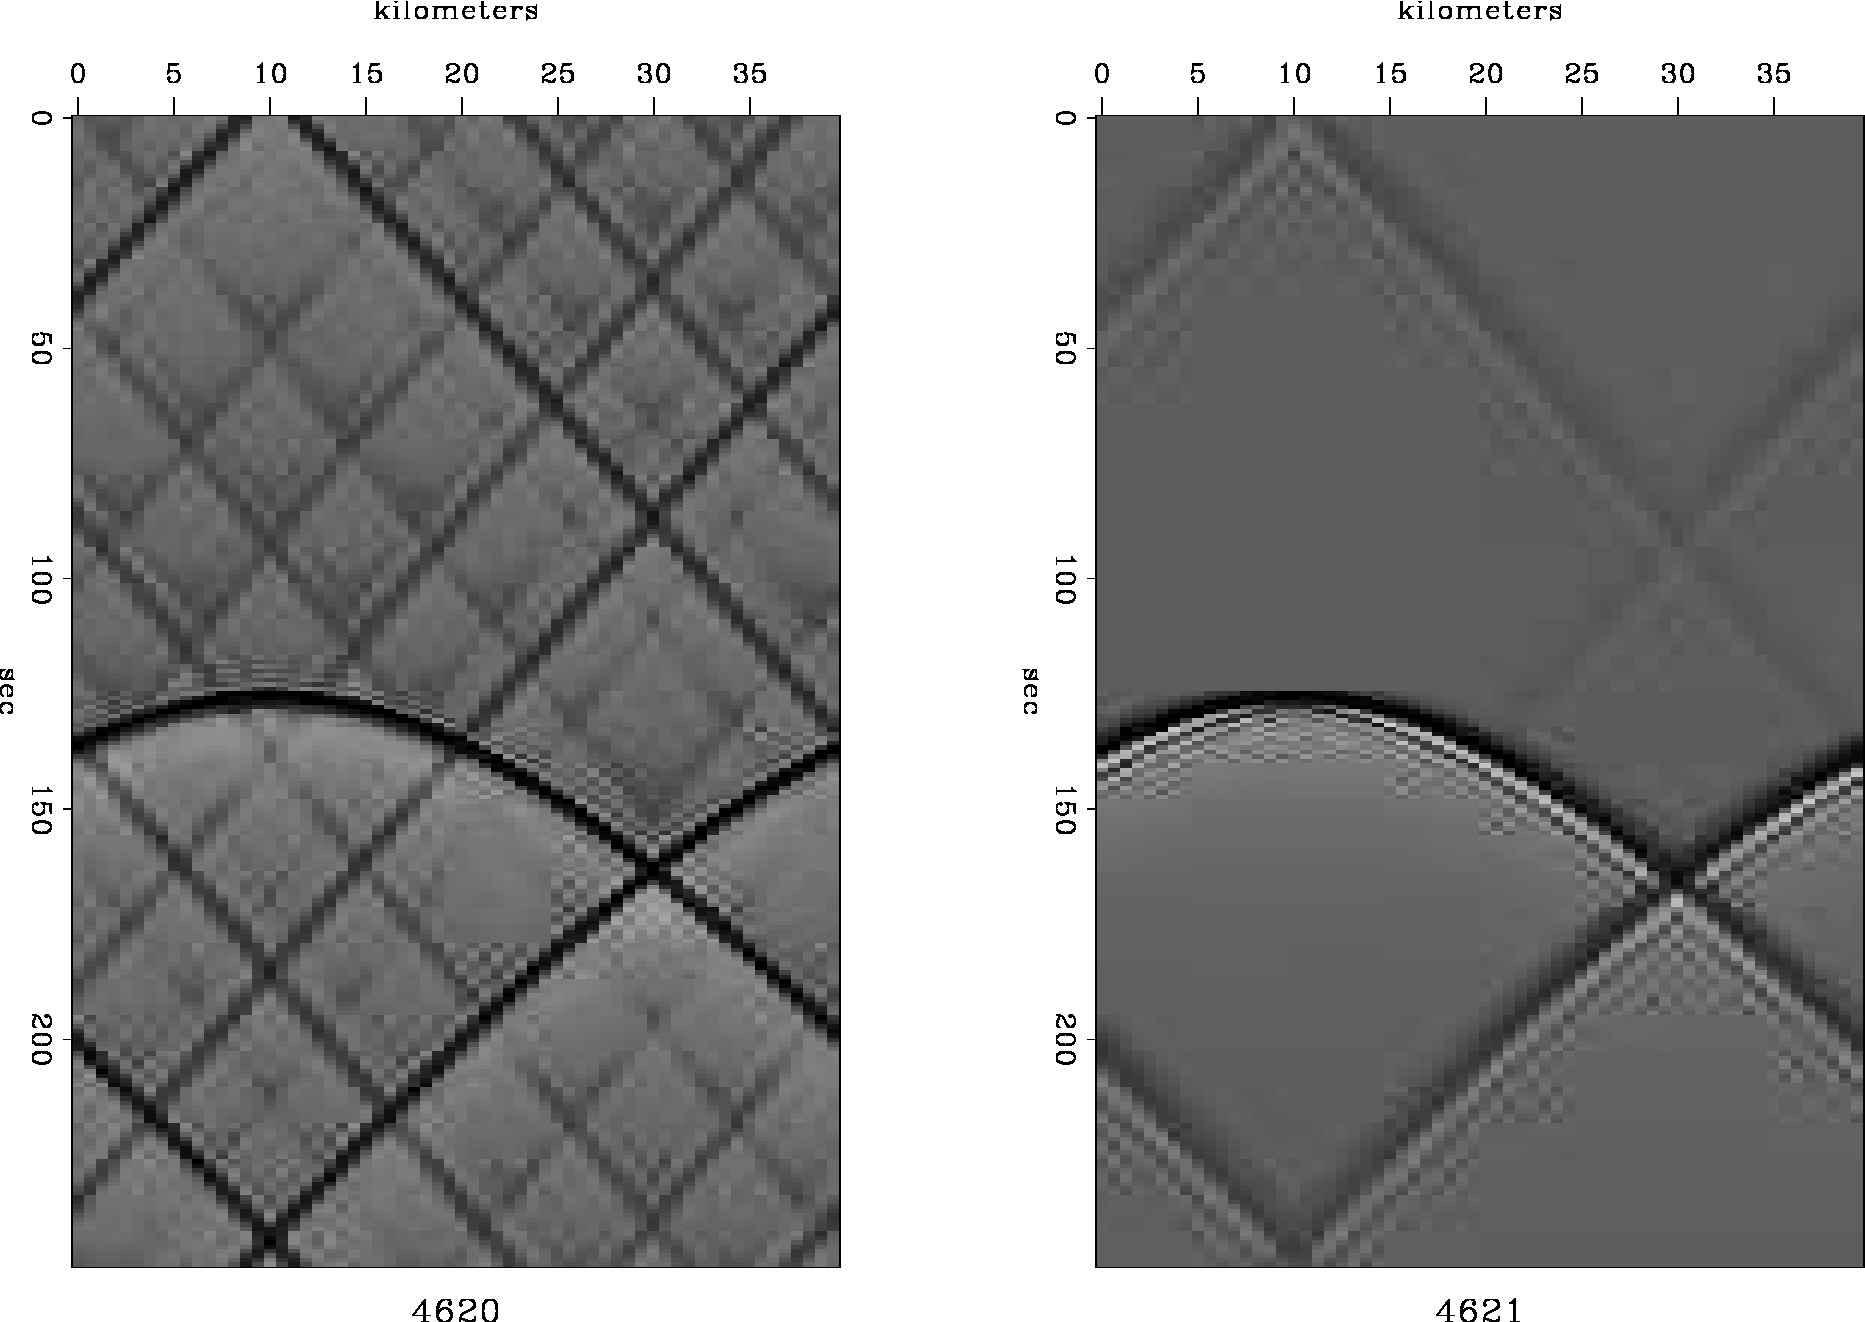
\includegraphics[width=0.65\textwidth]{crft/cxfreq}
\caption[cxfreq]{按实频率构制的双曲线(左图)和按复频率构制的双曲线(右图)
显示时,采用\ref{sec:4.1}节所述平方根增益}
\label{fig:crft/cxfreq}
\end{figure}

考虑下列由$R_0=s$开始的递归算法
\begin{equation}
R_{n+1}=s+\frac{X^2}{s+R_n}
\label{eq:ex4.6.30}
\end{equation}
这种递归产生的是连分式,Francis
Muir曾将它引入作为建立偏移的广角平方根近似时的
工具(见\ref{sec:2.1}节),而且他为表明每个均是一种阻抗函数而建立了他的三条规则。要想明白为
什么每种均为阻抗函数,首先得注意,从$n=0$时开始,分母$s+R_n$都是两个阻抗函数之和,
于是它的倒数应是一种阻抗函数。用正值实常数$X^2$乘和加上另一个s后全都保持着阻抗函数
的性质,如此循环作下去,我们将看到,所有的$R_n$都是阻抗函数。当n变大时,这种递归不
是收敛就是发散,假设它是收敛,令$R_{n+1}=R_n=R_{\infty}=R$我们就能知道它为什么会收敛。于
是
\begin{subequations}
\begin{equation}
R=s+\frac{X^2}{s+R}
\label{eq:ex4.6.31a}
\end{equation}
\begin{equation}
R(s+R)=s(s+R)+X^2
\label{eq:ex4.6.31b}
\end{equation}
\begin{equation}
R^2=s^2+X^2
\label{eq:ex4.6.31c}
\end{equation}
\begin{equation}
R=\sqrt{s^2+X^2}
\label{eq:ex4.6.31d}
\end{equation}
\end{subequations}

在波场外推问题中,$X^2$就是$v^2k_x^2$,其中v为波速,$k_x$为水平空间波数、即水平x坐标的
Fourier变换对偶。进行这些代换,我们得
\begin{equation}
R=\pm \sqrt{-\hat{\omega^2}+v^2k_x^2}
\label{eq:ex4.6.32}
\end{equation}
由此可知R类似于$\pm ik_zv$。记住,$R_0$作为对R的一级近似,就是$-i\hat{\omega}$。所以下行波为
\begin{equation}
D(x,z,t)=D(x,0,t)e^{ik_x}e^{-Rz/v}e^{-i\omega t}
\label{eq:ex4.6.33}
\end{equation}
为从下行波改换为上行波,我们可以改变R前面的符号,或者我们取R的复共轭,其差别就
看你要怎么处理实部---你要这个波增长还是不增长?

考虑一下波在爆炸反射面模型中的耗散。波随着自爆炸源至地面的传播而阻尼,这意味
着我们对波进行偏移时,它们应作指数式増长。可是,我们实际上并不想要它们这样,我们
真正想要的是保证它们不要增长,我们多半甚至是想使它们随着我们将它外推回去而阻尼。
所以,为进行偏移,我们是利用下式将单频菠向下延拓
\begin{equation}
U(x,z,t)=U(x,0,t)e^{ik_xx}e^{-\bar{R}z/v}e^{-i\omega t}
\label{eq:ex4.6.34}
\end{equation}
尽管由爆炸反射面产生的波其实际性态应为